% !TEX root = ../../main.tex
%

\chapter{Background} \label{chap:background}

\minitoc

Concurrency control is a crucial component in systems where multiple processes or threads simultaneously access shared resources, such as data structures, database tables, and system resources. Effective concurrency control mechanisms employ various synchronization techniques to maintain the safety and consistency of these shared resources. As noted by \citet{DBLP:books/daglib/0030596}, "Synchronization is a set of rules and mechanisms that allows the specification and implementation of sequencing properties on statements issued by the processes so that all the executions of a multiprocess program are correct."

In this chapter, we provide an introduction to multi-granularity locking. We discuss the structure of a hierarchy and the operations that can be performed on hierarchical data structures. We discuss the challenges brought forth by hierarchical data structures and the need for specialized locking techniques to manage concurrent access to them. 


% In this chapter, we provide an overview of concurrency control mechanisms, focusing on locking. We introduce a few classical locking mechanisms, their role in synchronization and in ensuring data consistency. We discuss additional challenges brought forth by hierarchical data structures and the need for specialized locking techniques to manage concurrent access to them. Finally, we introduce the concept of multi-granularity locking and its role in balancing the trade-offs between the extremes of locking in hierarchical data structures.


\section{Hierarchical data structures}

Hierarchical data models, which have their roots in the early days of computer science, play a critical role in the representation and storage of structured information. The inception of hierarchical data can be traced back to the 1960s with the development of the Information Management System (IMS) by IBM \cite{IBMIMS}. IMS was one of the earliest database management systems designed specifically for organizing hierarchical data and was initially created to manage the complex manufacturing data associated with the Apollo space program. IMS establishes a well-defined parent-child relationship between data entities, which is a defining characteristic of hierarchical models \cite{DBLP:books/daglib/0006734}.

Over the decades, hierarchical data structures have remained pertinent, particularly in domains that require nested or tree-like relationships. They are widely utilized in XML data management, file system hierarchies, and organizational charts \cite{DBLP:books/mk/BunemanSA99}. The relevance of hierarchical models has only increased in contemporary big-data contexts, where they are often integrated with other data models, such as graphs, to address the challenges posed by the complexity and interconnectedness of modern data environments.

For instance, hierarchical data models are fundamental in NoSQL databases like Apache HBase, where the efficient storage and rapid retrieval of large-scale, semi-structured data are critical \cite{DBLP:books/daglib/0027893}. The structured nature of hierarchical models aligns well with applications in social networks, content management systems, and cloud-based storage solutions, where understanding and managing data relationships is essential.
Consequently, hierarchical data models remain foundational to modern computing, providing an effective framework for organizing and retrieving complex, nested information.

\subsection{Structure of a Hierarchy}
A hierarchy is a tree like structure with an additional property that a vertex can have multiple parents.
Formally, a hierarchy is defined as follows:

\begin{definition}
    A hierarchy is a directed graph H=(V, E, R) and R $\in$ V where
    \begin{itemize}
        \item V is a finite set of vertices.
        \item $E \subset V \times V$ is a set of directed edges where each edge (u,v) represents a parent-child relationship between vertices u (the parent) and v (the child).
        \item R is the designated root of the hierarchy such that there is a path from R to every other vertex in V.
        
    \end{itemize} 
\end{definition}

\subsection{Data in Hierarchical data structures}

Hierarchical data structures are used to represent data that has a natural hierarchical relationship. This data is stored in the form of key-value pairs. Each vertex in a hierarchy has a unique identifier, type and set of attributes. The data stored in the vertices can be of any type, ranging from simple data types like integers and strings to complex data types like arrays and objects. 

Vertices are connected by edges that represent the relationships between them. These relationships are directional and often labelled. The labels on the edges can be used to represent the type of relationship between the vertices. For example, in a file system, the edges can be labelled as "contains" to represent the relationship between a directory and the files it contains. Figure \ref{fig:hierarchicalDS} shows an example of a hierarchical data structure with data on vertices and edges. In this hierarchy, vertices represent entities of type "Person". Each person has a unique identifier and the amount of food they possess. Person vertices are connected to each other via edges labelled \texttt{:isFriendTo} with a weight representing the strength of the friendship. So, we can infer that \emph{"Asterix is close friends with Obelix and a casual friend with Getafix"}.


\begin{figure}[h]
    \centering
    \captionsetup{justification=centering}
    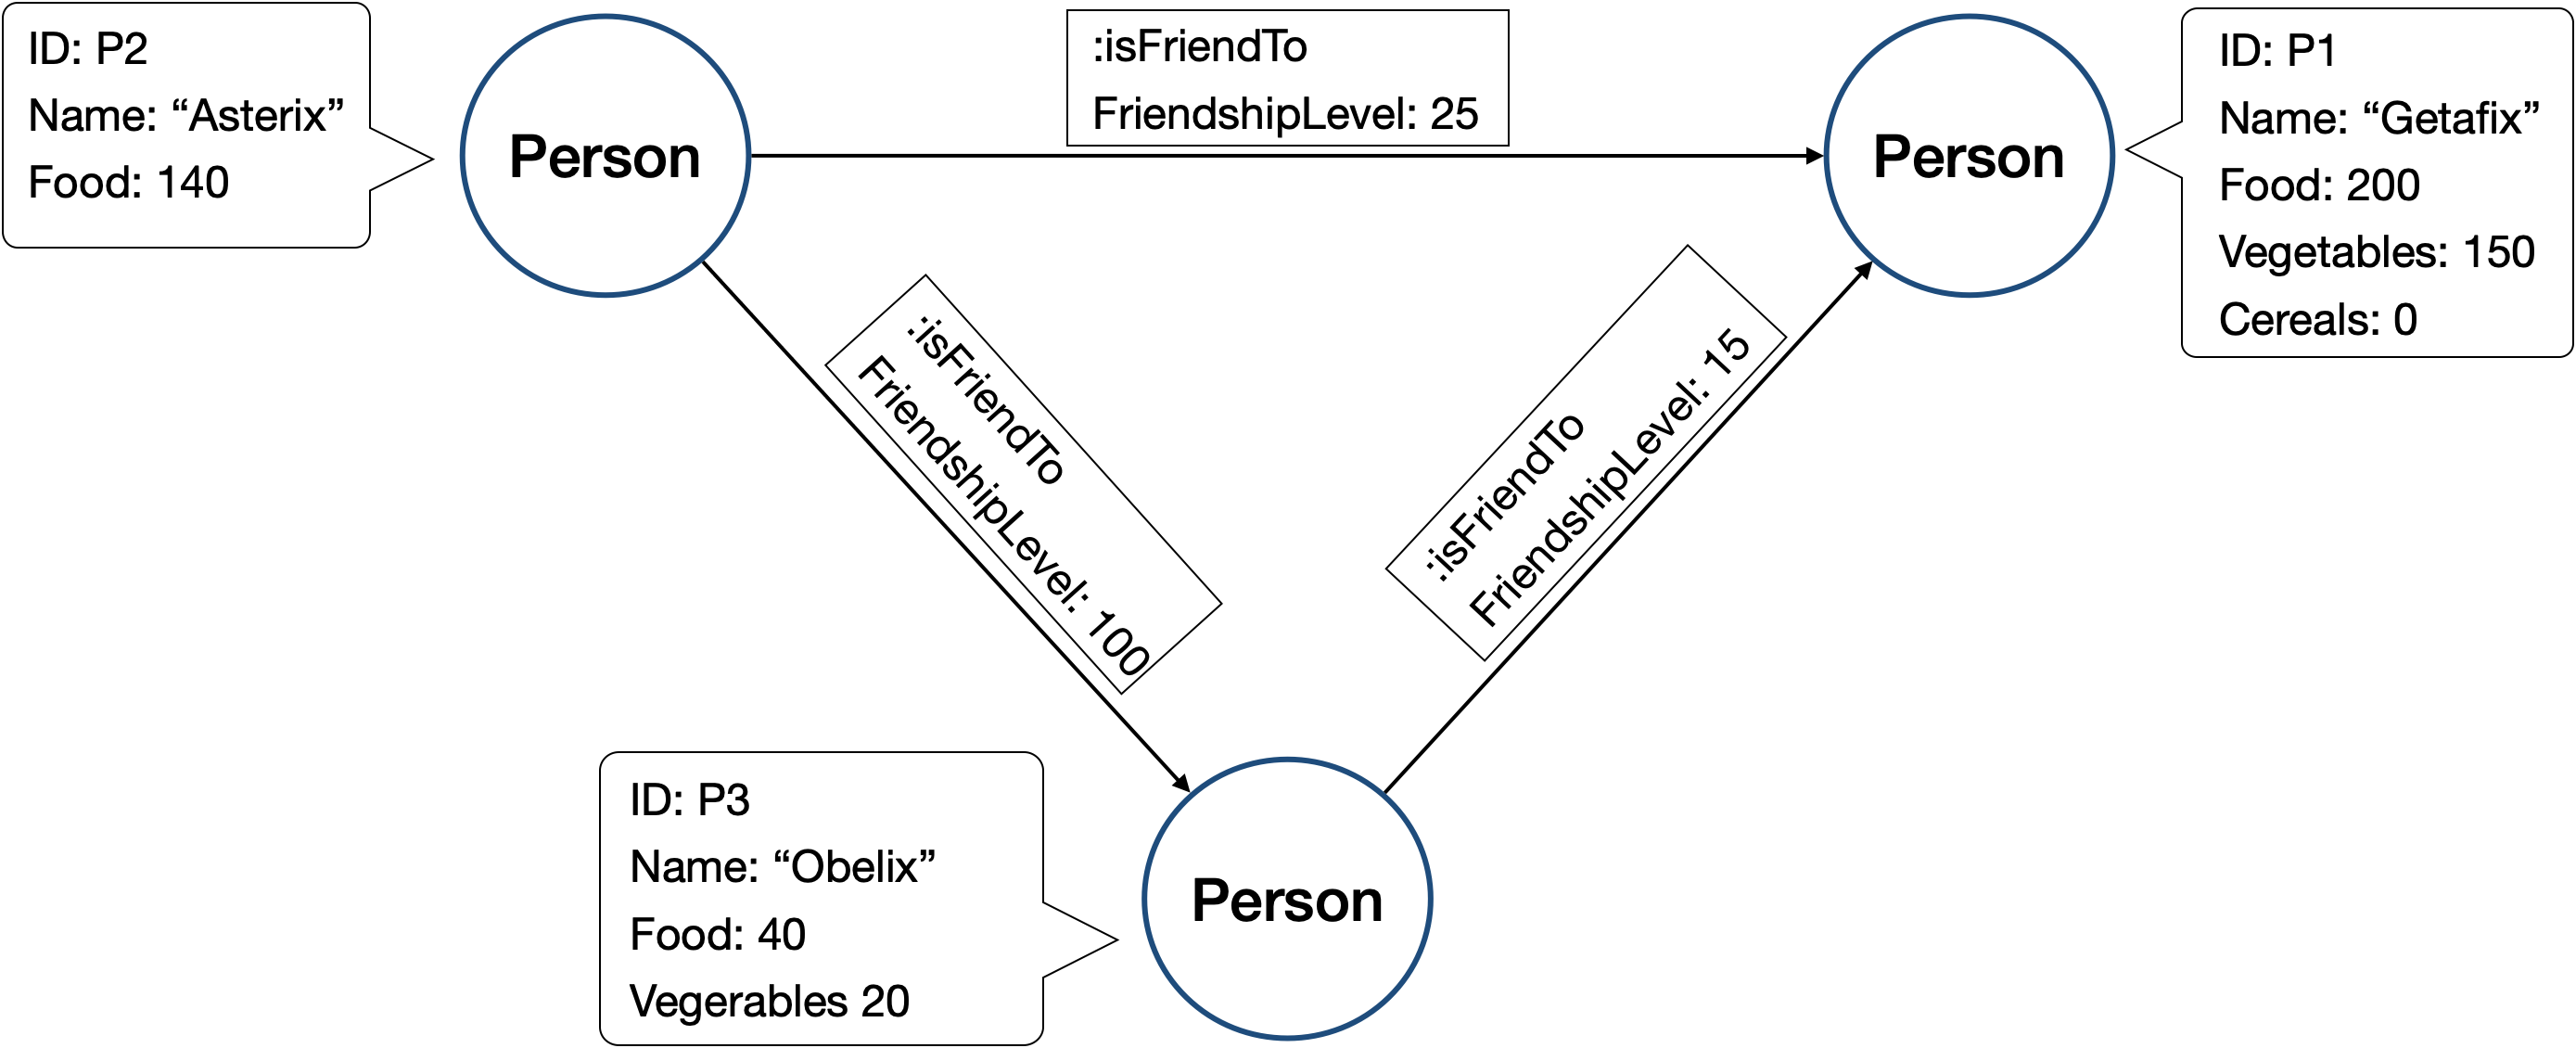
\includegraphics[width=\textwidth]{figures/HierarchicalDSExample.png}
    \caption{An example of a hierarchical data structure with data on vertices and edges.}
    \label{fig:hierarchicalDS}
\end{figure}




\subsection{Operations in Hierarchical Data Structures}

Hierarchical data structures support a variety of operations that enable querying and modification of the data. These operations are essential for managing data in the vertices and relationships between vertices of the hierarchy. Common operations on hierarchical data structures fall into two categories:

\begin{itemize}

    % \item \textbf{Search and Query:} Searching and querying operations involve locating specific vertices or paths within the hierarchy based on predefined criteria. These operations are essential for retrieving relevant information from the data structure. These operations result in read-only access to the hierarchy. While Data reads focus on vertices, search and query operations focus on relationships between vertices and use the edges to navigate the hierarchy.
    
    \item \textbf{Data Read and Write:} A data read and write operation involves accessing and/or updating attributes of vertices in a hierarchy. These operations are fundamental for interacting with the data and retrieving information from the structure. Often, one or more vertices are involved in a single read or write operation, depending on the specific requirements of the application. These operations do not alter the topology of the hierarchy.

    \item \textbf{Structural Modifications:} Inserting and deleting vertices or edges in a hierarchical structure can alter the observable topology of the hierarchy. These operations are crucial for creating new data and maintaining the integrity of the relationships between vertices. We call such operations \emph{structural modifications}.
    

\end{itemize}

\section{Locking, Consistency and Performance}
The primary goal of a multi-granularity locking protocol is to find an effective way of locking an entire \emph{sub-graph}. In a hierarchy, each vertex can be locked individually. This can be done to read or write the data on the vertex. However, in many applications, it is sometimes necessary to lock an entire sub-graph to ensure that the data remains consistent. For example, in a file system, it is necessary to lock an entire directory to ensure that the files within the directory are not modified by another concurrent thread.


When write locked, the requestor has exclusive access to a vertex and implicitly to all its descendants. When read locked, a requestor has shared access to the vertex and implicitly to all its descendants. Since MGL aims to lock entire sub-graphs, it is essential to prevent another transaction from acquiring a lock on a vertex that is an ancestor of a locked vertex. Assume a vertex $v$ is locked in write mode. This implicitly locks the entire subtree rooted at $v$ in write mode. If another transaction acquires a lock on an ancestor $a$ of $v$, the sub-graph rooted at $a$, which also contains the sub-graph rooted at $v$, is implicitly locked. This violates the core invariant of MGL, which is to provide isolated access of sub-graphs to threads. To prevent this, MGL must ensure that no ancestor of a locked vertex is locked by another transaction. 
% This is achieved by ensuring that the lock request for a vertex $v$ is blocked if any descendant of $v$ is locked by another transaction.

An important concern of an application, after correctness, is performance. Performance of a correct locking protocol is determined by the rate at which locks can be granted i.e. \emph{locking throughput}. A correct application that is slow is, often, not useful in practice. In database design, this performance is driven by the choice of \emph{lockable units}. A lockable unit is a set of data which should be atomically locked to ensure data consistency. A smaller lockable unit allows for more concurrency and better performance if transactions are simple i.e., do not access a lot of data items. Complex transactions access several data items and incur a lot of overhead in acquiring and releasing locks. In such cases, a larger lockable unit is more efficient as it reduces this overhead.  On the other hand, to ensure consistency, a larger lockable unit discriminates against transactions that access only a few data items by requiring them to wait. It is therefore desirable to vary the size of this lockable unit based on the access requirement of a transaction and have varying sizes of lockable units in the system. This is the motivation behind multi-granularity locking. 

\section{Multi-Granularity Locking: Terminology and Concepts}
In this section, we introduce the key concepts and terminology associated with multi-granularity locking (MGL) in hierarchical data structures. These concepts are essential for understanding the challenges and solutions presented by MGL protocols.
In particular, concepts like "lock grain," which describe the lockable units in hierarchical locking, are critical for understanding the nuances of how concurrency is managed in graph-based data models. While some of these terms are standard in the literature, others are specific to the context of this thesis, reflecting the unique challenges and solutions presented by hierarchical data structures.


\paragraph{Lock Target} The lock target refers to a specific vertex or a set of vertices within the hierarchy that a transaction accesses. A transaction may access a single lock target or a set of them. A lock target is defined independently of a locking protocol.  

\paragraph{Lock Guard} The lock guard is an entity that serves as the point of synchronization for a given set of lock targets. When a thread wishes to access a particular target, it must acquire the corresponding lock guard to ensure data consistency. The lock guard acts as a sentinel, preventing other threads from modifying the protected data until the lock is released. The mapping between a lock target and its corresponding lock guard is dependent on the locking protocol. We shall see examples of this in Chapter \ref{chap:relatedwork}.

\paragraph{Lock Grain} Lock grain refers to the scope of the data that is being locked when a lock is acquired on a guard. In multi-granularity locking, a lock grain is the lockable unit which is protected by locks. A grain is rooted at a vertex and includes all descendants of that vertex. This root is designated as the lock guard for the grain.

\paragraph{Granularity} The size of the grain is called its \emph{granularity} which varies from coarse-grained locks that encompass large portions of the hierarchy (e.g. entire sub-graphs) per lock guard to fine-grained locks that target individual vertices or smaller groups of vertices per lock guard. The choice of lock grain (resp. granularity) directly impacts the level of concurrency and performance in a system; while fine-grained locks allow for greater parallelism, they can introduce additional complexity in managing locks.

\subsection{Access Modes and Conflicts}

MGL protocols lock grains in either read or write mode. A read lock on a grain allows other transactions to acquire read locks on the same grain but prevents any transaction from acquiring a write lock. A write lock on a grain prevents any other transaction from acquiring a read or write lock on the grain.
Two lock requests are compatible with each other if they can be granted concurrently. In MGL, this compatibility is determined by two conditions: \textbf{mode conflict} and \textbf{grain conflict}. 

A mode conflict is dependent on the semantics of the lock. MGL uses the standard read/write lock semantics. A write lock guarantees lock grain exclusivity and is incompatible with any other lock request. A read lock allows shared access to a grain and is compatible with other read locks but not with write locks. Some MGL protocols, like intention locks, further develop this concept by introducing additional modes to indicate the intent of a transaction to acquire a lock in a specific mode before an actual lock is acquired. An intention lock, thus, is not compatible with a read or write lock. 

A grain conflict occurs when two lock requests target overlapping grains. The grain of a lock request is a set of vertices protected by a guard. If the grains of two lock requests have vertices in common, then they conflict. Different MGL protocols have different strategies to detect grain conflicts. Intention locks use a deterministic DFS traversal combined with intention locks to prevent grain conflicts. Others, as we discuss in Chapter \ref{chap:relatedwork} use labelling schemes.


\section{Acquiring MGL Locks in a Hierarchical Data Structure} \label{sec:lockAcquisitionProtocol}
MGL protocols implicitly lock sub-graphs rooted at a lock guard. If transactions are allowed to randomly access vertices in the hierarchy, grain conflicts will remain undetected and cause data inconsistency. To prevent this, MGL protocols, often, assume a defined order of operations for lock acquisition. 

\begin{enumerate}
    \item \textbf{Optional preprocessing:} Preprocessing is a one-off step required for certain MGL protocols to prepare a hierarchy for lock acquisition. During preprocessing, metadata required for a locking protocol to function is computed. This metadata, often stored in the vertices of the hierarchy, is then used to optimize lock grain identification and conflict detection. 
    \item \textbf{Preparing a lock request:} Once a transaction identifies the set of data it wishes to access, it must prepare a lock request. This request must include information to at least identify the lock grain and the lock mode. Different MGL protocols may require additional information as we discuss in Chapter \ref{chap:relatedwork}.
    \item \textbf{Requesting a lock:} Once a lock request is prepared, it is submitted to the scheduling mechanism of the locking protocol that decides whether to grant the lock request or block it. If blocked, the transaction waits until it is notified to resume. When granted, the transaction proceeds to perform the operation on the vertices. The locks are granted in a deterministic order, often from the root to the leaves of the hierarchy. This is done to guarantee that no ancestor of a locked vertex is locked by another transaction. 
    \item \textbf{Performing an operation:} Once a lock is granted, the transaction can access the locked grain. The transaction may read/write data on the vertices or perform structural modifications by adding/removing edges. Since the grain is isolated from other transactions, any changes made by the transaction are not visible to other transactions until the lock is released.
    \item \textbf{Optional metadata maintenance:} For protocols that use metadata to identify grains, the transaction may need to update this metadata to reflect the changes made to the hierarchy. For example, if a vertex is deleted, the metadata must be updated to reflect this change. Not all MGL protocols require this step.
    \item \textbf{Releasing the lock:} Once the transaction completes its operation, it releases the lock on the grain. This makes the updates visible to other transactions. This grain is now available for other transactions to lock and access. Locks should be released from the leaves to the root to ensure an ancestor is not unlocked before its descendants are unlocked.
\end{enumerate}



% \section{Need for Concurrency Control in Hierarchical Data Structures} \label{sec:multicoresystemsandconcurrencycontrol}
% Locking mechanisms in hierarchical data structures are essential for ensuring data consistency and integrity in concurrent environments where multiple processes or threads may attempt to access or modify data simultaneously. Given the inherently nested and interdependent relationships among vertices in hierarchical structures, specialized locking techniques are often required to effectively manage concurrent access.

% The primary objective of locking in these structures is to prevent race conditions, which occur when two or more operations interfere with one another, potentially resulting in an inconsistent or incorrect data state. By implementing appropriate locking strategies, it is possible to coordinate access to shared resources, thus safeguarding the integrity of the data and maintaining the correctness of operations performed within the hierarchy.

% This work on locking focuses on a multicore system where threads concurrently access a shared graph. Such use-cases provide the possibility to use a single centralized scheduler which decides on the ordering of the lock requests. In distributed deployments like HPC clusters where the communication can be guaranteed to be quasi-instantaneous, locking can still be useful since synchronization primitives can be implemented without worrying about catastrophic network partitions. Geo-distributed graphs and synchronization are out of the scope of this work. As such, locking in any form is not an efficient solution for use-cases where the graph is geo-distributed and the communication latency (ergo the synchronization delay) is high. 

% The requirement for any locking technique over graphs is to protect the vertices and edges of the graph against concurrent write access. Writes can modify the data on the vertices or add/remove edges from the graph. 

% A lock protocol typically involves five main steps:

% \begin{enumerate}
%     \item \textbf{Requesting a Lock:} A thread initiates the locking process by submitting a request to acquire a lock on a specific set of vertices that it intends to access for a write operation. This request is an attempt to ensure that only the requesting thread can modify said vertices during the operation, thereby maintaining data integrity and avoiding interference from other concurrent operations.

%     \item \textbf{Detecting Conflicts:} Upon receiving a lock request, the locking protocol detects conflicts with locks held by other threads. This step is critical to preserve mutual exclusion. If a conflict is detected, the protocol determines whether the requesting thread should proceed or be temporarily blocked.


%     \item \textbf{Acquiring a Lock:}  If conflict detection confirms no overlapping locks, the locking protocol grants the requested lock, allowing the thread to proceed with its intended write operation. In cases where a conflict exists, the requesting thread is put into a blocked state, where it waits until the conflict is resolved, typically by the release of the conflicting lock. This blocking mechanism is designed to prevent busy-waiting and reduce system resource usage.

%     \item \textbf{Performing an Operation:} With the lock granted, the thread performs its designated read or write operation on the locked vertices. The lock ensures that no other thread can access these vertices concurrently for a write operation. Upon completing the operation, the thread prepares to release the lock, signaling the end of its exclusive access.
    
%     \item \textbf{Releasing the Lock:} After finishing the operation, the thread releases the lock on the vertices, allowing other threads to request and potentially acquire locks on the same vertices. This release phase reopens access to the locked vertices, ensuring that other threads waiting to modify or read the same graph segments can proceed according to the locking protocol's scheduling and prioritization rules.
% \end{enumerate}

An implementation of a locking protocol makes a few assumptions on the implementation and use.

\begin{enumerate}
    \item \textbf{Atomicity of Lock Operations:} We assume that lock acquisition and release operations are atomic, meaning they are indivisible and cannot be interrupted mid-operation. This atomicity ensures that no two threads can simultaneously acquire a lock on the same Grain.

    \item \textbf{Cooperating Threads:} The algorithm assumes that threads behave cooperatively, without attempting to bypass or tamper with the locking mechanism. This assumption excludes scenarios where threads might act maliciously or fail to adhere to the locking protocol, simplifying the conflict detection and lock management processes.
    
    \item  \textbf{Fairness in Lock Scheduling:} Many locking algorithms assume a fair scheduler, meaning that a lock request is eventually granted in finite time, avoiding starvation where certain threads are indefinitely blocked. Fairness ensures that all threads have equitable access to shared resources.

    \item \textbf{Deterministic Conflict Detection:}  It is assumed that the conflict detection mechanism can deterministically identify conflicts between lock requests and consistently enforce access restrictions. This assumption is crucial for ensuring that threads either proceed with their operations or are correctly blocked when a conflict is detected.
    
    \item \textbf{Consistency of Shared State:} The algorithm assumes that the state of shared data remains consistent and is correctly updated before each lock release. This assumption ensures that subsequent transactions access a consistent version of the graph data, preventing issues such as stale data reads or lost updates.
\end{enumerate}


Together, these prerequisite steps and assumptions form the foundation for effective concurrency management, allowing the locking algorithm to maintain data integrity while maximizing system efficiency.



\section{Design Guideline for a Multi-Granularity Locking Protocol} \label{sec:requirements}

A lock protocol based on the steps described in Section \ref{sec:lockAcquisitionProtocol} performs three key functions: Identifying the lock grain, detecting conflicts between lock requests, and managing the metadata required to implement the locking protocol. Each of these can be optimised to improve the throughput of the system. However, these optimizations are often at odds with each other. As we will describe in more detail in Chapter \ref{chap:relatedwork}, a lock protocol that uses a deterministic traversal to detect conflicts can achieve smaller grains but incurs a higher penalty in terms of identifying lock conflicts. On the other hand, a lock protocol which eliminates traversals all together, using metadata to detect conflicts, needs to optimize the metadata management to increase throughput. The three primary requirements of a correct MGL technique are:

\begin{itemize}

    \item[\Rb] \emph{Finding an appropriately sized grain for a request}. When a thread requests a lock on a set of lock targets, a locking protocol must determine a lock grain for this request such that a lock on said grain maximizes throughput. This involves considering the topology of the hierarchy and the relationships between vertices to minimize grain conflicts.
    
    \item[\Rc] \emph{Efficiently detecting conflicts between locks}. Mode conflicts and grain conflicts between lock requests must be detected correctly to guarantee data consistency and efficiently to improve lock throughput. Mode conflicts can be detected by maintaining a lock table that records the lock mode for each transaction. Grain conflicts are more complex and often require sub-graph traversal to identify overlapping grains. A lock protocol must ensure that a locked grain is not accessed by a transaction with a conflicting mode. Several MGL protocols use additional metadata to optimize detecting grain conflicts.
    
    % Since a correct locking protocol is workload agnostic, it must allow a thread to efficiently detect conflicts with other lock requests. In MGL, this involves testing the ancestor-descendant relationships between two lock guards which in turn implies grain overlap. If a thread requests a lock on a vertex, then to prevent conflicts, a locking protocol must ensure that no ancestor or descendant of this vertex is locked by another thread in a conflicting mode. 
    
    \item[\Rd] \emph{Housekeeping the metadata required to implement the locking protocol.} The additional metadata required to implement the locking protocol and the conflict detection mechanism must be managed efficiently to minimize the overhead of using that particular locking protocol. If the metadata management is prohibitively expensive for certain workloads, the locking protocol may not be practical for real-world applications that encounter those workloads. 

\end{itemize}


The goal of a correct MGL technique is to maximize throughput. This throughput is measured by the number of lock requests that can be granted in a unit of time. Depending on the lock protocol, this can translate to an optimization of the former three requirements. For example, a lock protocol that uses a deterministic traversal to detect conflicts can detect conflicts more efficiently by implementing graph-isomorphism tests. This, in turn, increases the throughput of the system but incurs a higher memory footprint. A lock protocol that uses labelling, omits traversals all together and needs to optimize the metadata management to increase throughput. 

\begin{figure}[h]
    \centering
    \captionsetup{justification=centering}
    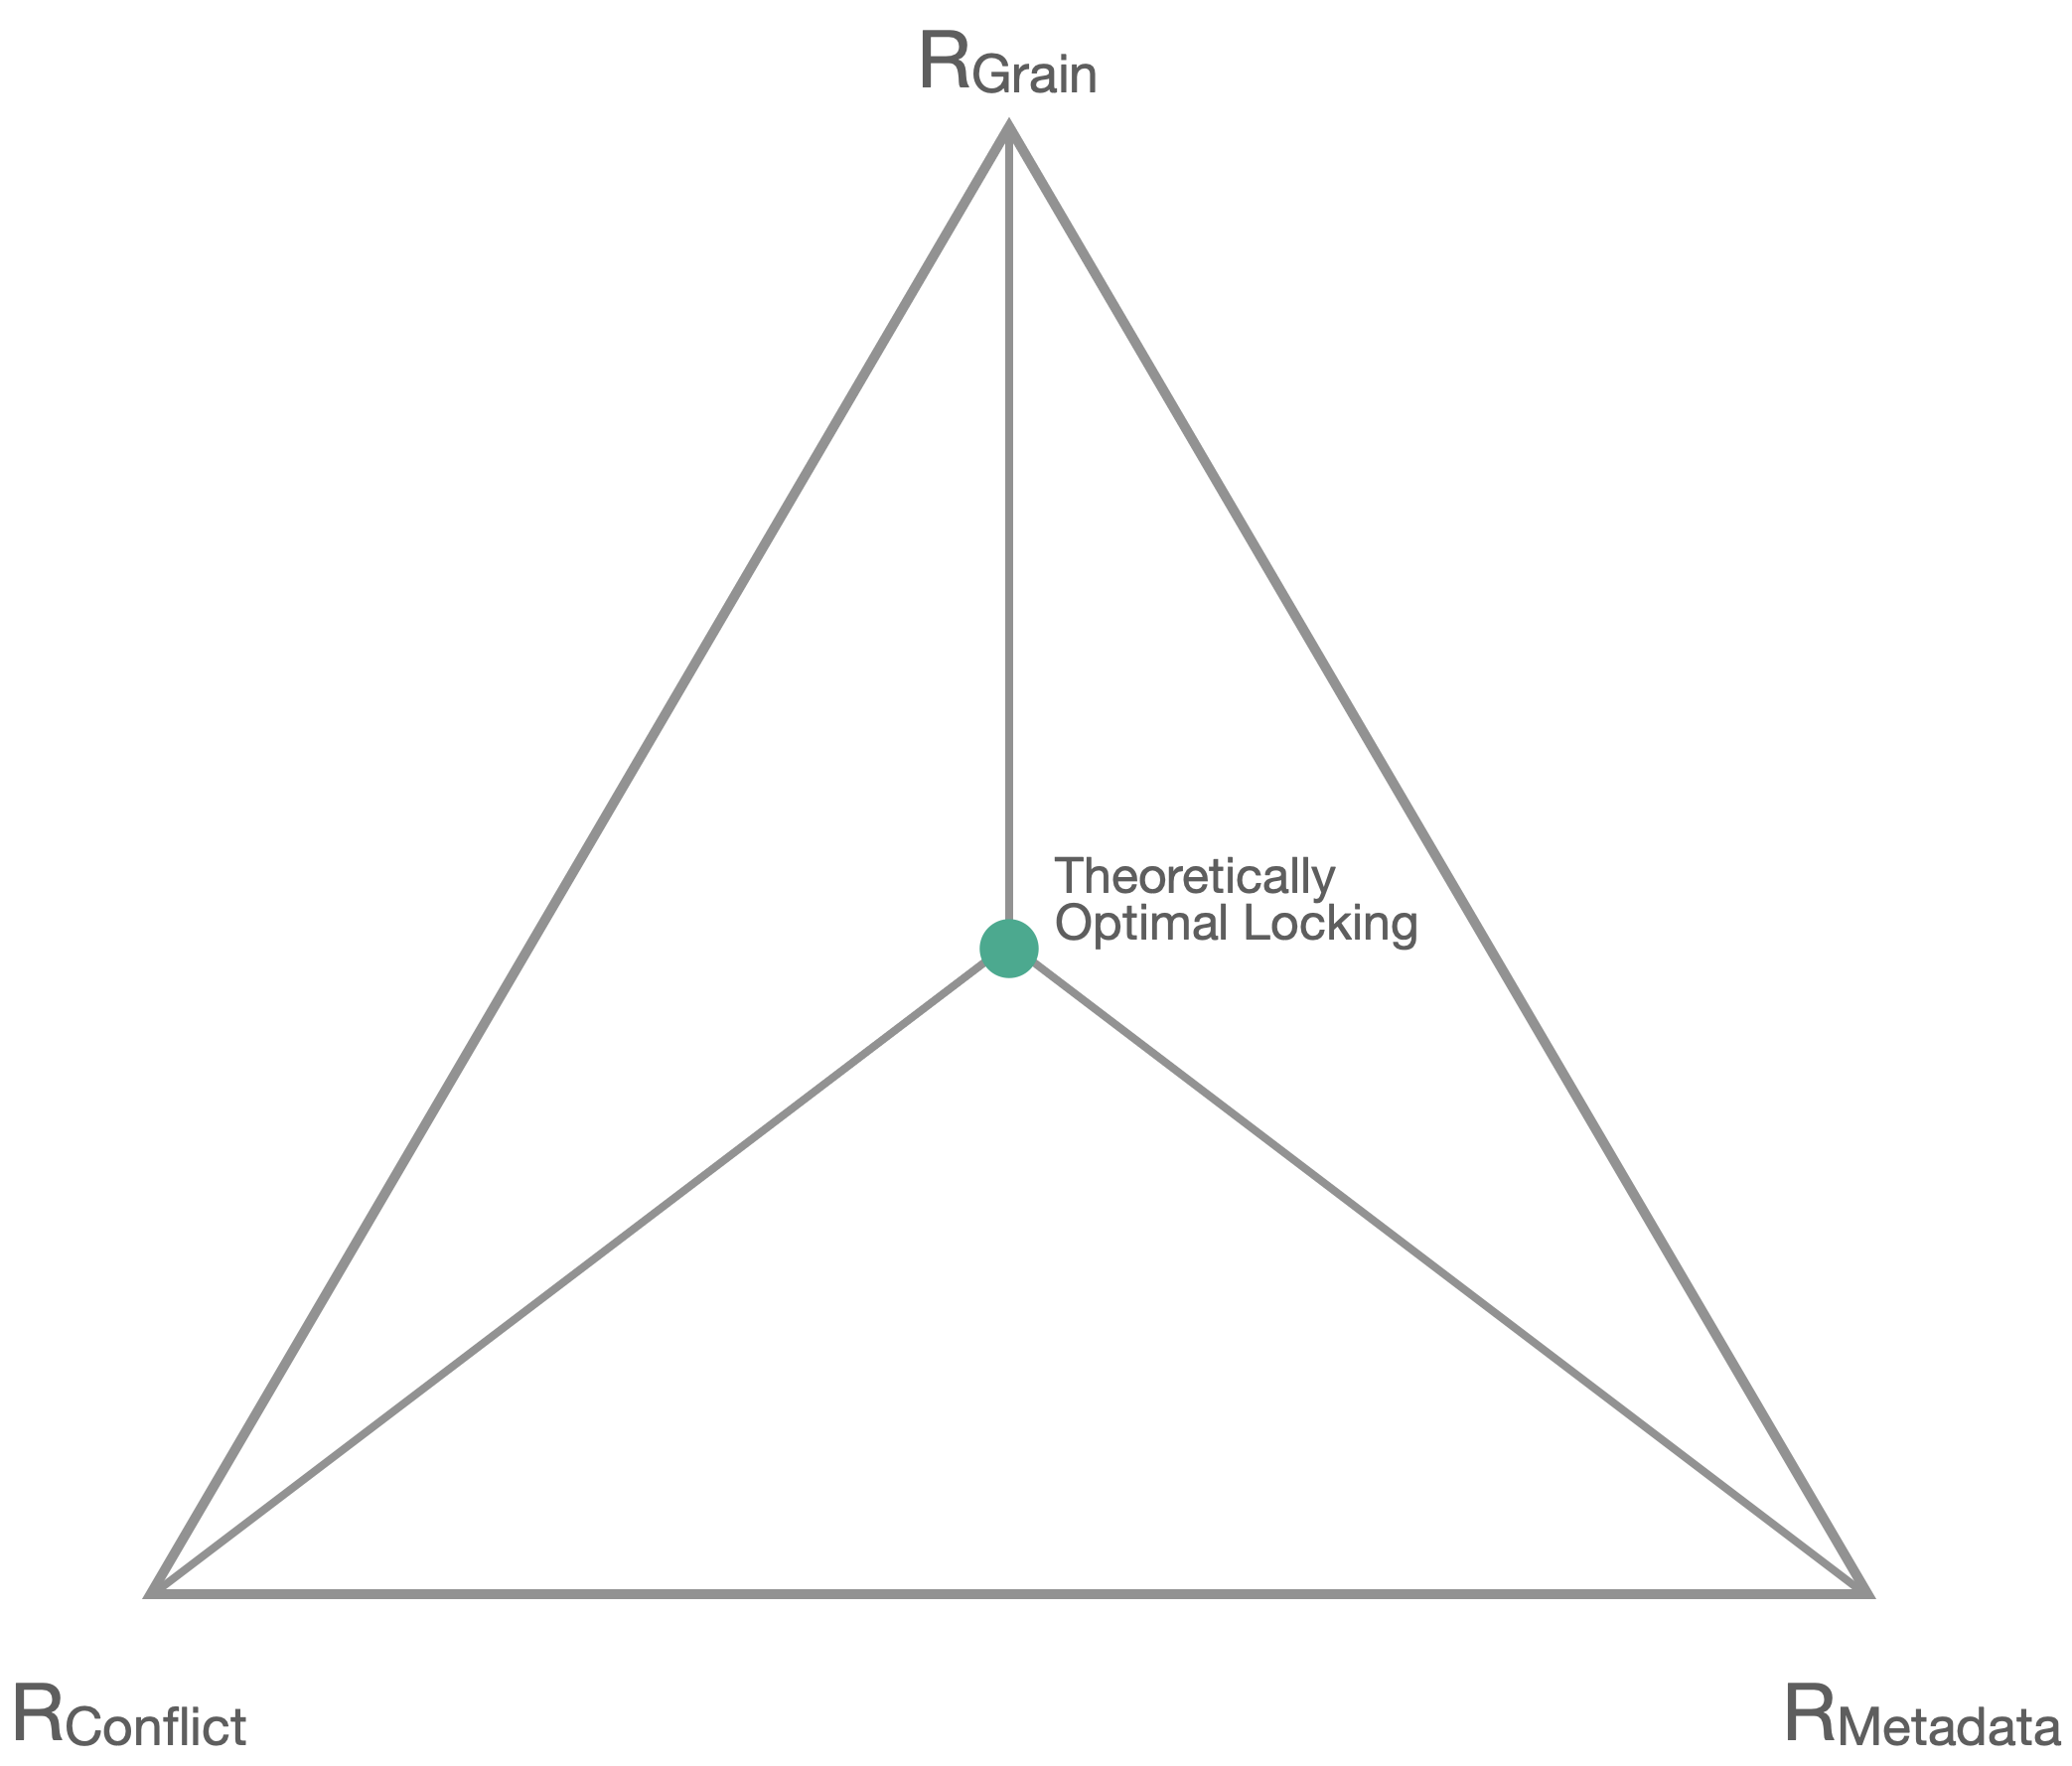
\includegraphics[width=0.8\textwidth]{figures/IdealMGLTechnique.png}
    \caption{An optimal MGL technique balances the trade-offs between the three requirements to maximize throughput.}
    \label{fig:lock_throughput}
\end{figure}



% An application that uses CALock can have multiple threads that concurrently access the graph. Each thread can request a lock on a set of vertices(lock targets). The locking algorithm then grants the lock request by locking a single vertex(the guard), that protects the set of vertices.
% Once a thread identifies a guard and issues a lock request, the guard cannot to be changed i.e. the guard is fixed for the duration of the lock. This is to ensure that the lock grain remains consistent for the duration of the lock. If a conflict is detected between two lock requests, one of the threads is blocked until it is notified to resume i.e. no busy waiting. In our design, we assume that the threads are not malicious and do not try to circumvent the locking and conflict detection mechanism



% \section{Role of Locking in Concurrency Control}
% As computing systems increasingly rely on concurrent processing, effective concurrency control mechanisms are essential for ensuring the integrity and reliability of shared resources. Locking mechanisms are a foundational strategy in managing access to these resources, allowing for mutual exclusion and preventing conflicts that can arise when multiple threads attempt to modify shared data simultaneously.

% In this section, we explore the critical roles that locking plays in concurrency control. We first examine how locks prevent race conditions by ensuring that only one thread can modify shared data at a time. Next, we discuss the importance of locks in maintaining data consistency through atomic operations. Finally, we address the challenges of deadlock prevention and the strategies that can be employed to minimize this risk. Through this overview, we highlight the significance of locking mechanisms in supporting robust and reliable concurrent programming.


% \subsection{Safety}

% Race conditions are a fundamental concern in concurrent programming, occurring when multiple threads access and modify shared data simultaneously without proper synchronization mechanisms in place. This lack of coordination can lead to unpredictable and erroneous outcomes, as the final state of the data may depend on the timing of the thread executions rather than a well-defined sequence of operations. Locks play a critical role in preventing race conditions by ensuring that only one thread can modify shared data at any given time. By acquiring a lock before accessing the data, a thread effectively prevents other threads from making concurrent modifications, thereby establishing a controlled environment for data access.

% The implementation of locks creates critical sections—regions of code that must be executed by only one thread at a time. When a thread acquires a lock, it enters the critical section and can safely perform operations on the shared data, knowing that no other thread can interfere during this period. Once the operations are complete, the thread releases the lock, allowing other waiting threads to enter the critical section. This mechanism not only prevents race conditions but also enhances the reliability of concurrent programs, as it provides a straightforward method for enforcing mutually exclusive access to shared resources.

% % \subsection{Ensuring Data Consistency}

% Locks are instrumental in ensuring data consistency across concurrent operations. In computing, consistency refers to the property that shared data remains in a valid state throughout the execution of concurrent transactions. Locks help maintain this consistency by enforcing atomicity, a key aspect of transaction management that dictates that operations on shared data should be treated as indivisible units. This means that a series of operations can either be completed in their entirety or not executed at all, effectively preventing intermediate states that could lead to data corruption.

% For instance, consider a banking application where a user initiates a transfer of funds from one account to another. This operation typically involves several steps: debiting the source account, crediting the destination account, and possibly updating transaction logs. If these operations are interrupted by another thread accessing the same accounts, the integrity of the transaction may be compromised, leading to scenarios such as double spending or incorrect balances. By using locks to protect these operations, the system ensures that each transfer is executed atomically, thus maintaining the integrity and consistency of the financial data. This mechanism is crucial not only for ensuring correctness in transactional systems but also for building trust in applications that rely on shared data.


% \subsection{Liveness}

% While locks are essential for ensuring safe and consistent access to shared resources, their improper use can lead to deadlocks—situations where two or more threads are waiting indefinitely for each other to release locks, thereby causing a standstill in program execution. Deadlocks can severely impact system performance and responsiveness, making it critical to implement strategies for their prevention.

% Several techniques can be employed to mitigate the risk of deadlocks in systems utilizing locks. One common approach is lock ordering, which mandates that all threads acquire locks in a predefined sequence. By adhering to a global order for lock acquisition, the system effectively eliminates circular wait conditions, which are a primary cause of deadlocks. For example, if Thread A acquires Lock 1 and Thread B acquires Lock 2, both threads should be programmed to request subsequent locks in the same order. This strategy significantly reduces the chances of deadlock occurrences, as it prevents the formation of cycles in the waiting graph.

% Another useful technique is the implementation of timeout mechanisms. By allowing threads to specify a maximum waiting period for acquiring locks, the system can reduce the likelihood of indefinite waiting. If a thread cannot acquire the desired lock within the specified time-frame, it can abandon its attempt and either retry later or perform alternative actions. This not only aids in breaking potential deadlocks but also enhances overall system responsiveness, as it prevents threads from being indefinitely stalled.



% \section{Requirements} \label{sec:requirements}



% \section{Concurrency control though general locking}
% The form of synchronization studied in our work is \emph{competition synchronization} where multiple threads compete for access to shared resources. 
% Locking is one of the primary mechanisms used to ensure data integrity and consistency in such environments.
% It restricts access to a shared data structure by multiple threads or processes to prevent conflicts and ensures that no more than one writer can modify the data at a time. 
% Here’s a high-level overview of how locking works and its role in concurrency control:

% \subsection{Mutex (Mutual Exclusion) Locks}

% One of the most fundamental forms of locking is the mutex lock, short for \emph{mutual exclusion} lock. A mutex lock is designed to provide exclusive access to a shared resource by ensuring that at most one thread can acquire the lock at any given time. When a thread requests a mutex lock, it must wait if another thread currently holds the lock. Once the holding thread releases the lock, the waiting thread can then acquire it, thereby gaining access to the shared resource.

% Mutex locks are widely used in various concurrent programming scenarios, as they effectively prevent race conditions—situations where the outcome of operations depends on the unpredictable timing of thread execution. By enforcing mutual exclusion, mutex locks ensure that critical sections of code, where shared resources are accessed or modified, are executed by only one thread at a time.

% \begin{lstlisting}
%     std::mutex mtx;
%     int counter = 0;

%     void increment(int iterations) {
%         for (int i = 0; i < iterations; ++i) {
%             std::lock_guard<std::mutex> lock(mtx);
%             ++counter;
%         }
%     }
% \end{lstlisting}

% While mutex locks are effective for synchronization, they also introduce potential drawbacks, such as lock contention and the risk of deadlocks. Lock contention occurs when multiple threads attempt to acquire the same mutex lock simultaneously, resulting in delays and reduced performance. Deadlocks can arise when two or more threads are waiting indefinitely for locks held by each other, creating a cycle of dependency.

% Mutex locks provide a straightforward mechanism for managing access to shared resources, although careful design is required to mitigate their inherent limitations.



% \subsection{Reader-Writer Locks}
% Another important synchronization mechanism is the reader-writer lock also called shared-exclusive lock. Reader-writer locks are designed to allow concurrent access to shared resources while differentiating between two types of operations: read and write. This differentiation facilitates improved performance in scenarios where read operations significantly outnumber write operations.

% A reader-writer lock enables multiple threads to simultaneously acquire the lock for reading, provided that no thread is currently writing. This means that as long as the resource is not being modified, multiple readers can access the resource concurrently, enhancing throughput. Conversely, when a thread intends to write to the shared resource, it must acquire exclusive access, which means that no other readers or writers can access the resource during this time. This mechanism prevents data inconsistency that could arise from simultaneous read and write operations.

% \begin{lstlisting}
%     ReaderWriterLock rwlock;
%     int counter = 0;

%     void reader(int iterations) {
%         for (int i = 0; i < iterations; ++i) {
%             rwlock.reader_lock();
%             // Read operation (e.g., print counter)
%             std::cout << "Read counter: " << counter << std::endl;
%             rwlock.reader_unlock();
%         }
%     }

%     void writer(int iterations) {
%         for (int i = 0; i < iterations; ++i) {
%             rwlock.writer_lock();
%             ++counter;
%             rwlock.writer_unlock();
%         }
%     }
% \end{lstlisting}

% The structure of reader-writer locks generally consists of two types of locks: a read lock and a write lock. When a thread requests a read lock, it can proceed if no write lock is held; however, if a write lock is active, the requesting thread must wait. When a thread requests a write lock, it must wait until there are no active readers or writers.

% While reader-writer locks can enhance performance by allowing multiple concurrent reads, they introduce complexity in terms of synchronization. One potential challenge is ensuring fairness, as a prolonged sequence of read operations could lead to writer starvation, where a waiting writer is indefinitely delayed because readers continue to acquire the read lock. Additionally, if not managed carefully, reader-writer locks can still suffer from lock contention and deadlocks.

% Reader-writer locks are powerful for optimizing access to shared resources, particularly in read-heavy environments. They allow for greater concurrency compared to mutex locks, but their implementation requires careful consideration to avoid potential pitfalls.



% Spinlocks:
% \begin{lstlisting}
%     Spinlock spinlock;
%     int counter = 0;

%     void increment(int iterations) {
%         for (int i = 0; i < iterations; ++i) {
%             spinlock.lock();
%             ++counter;
%             spinlock.unlock();
%         }
%     }
% \end{lstlisting}
% Spinlocks are a type of lock where a thread repeatedly checks if the lock is available, consuming CPU cycles.
% They are useful in scenarios where the wait time is expected to be very short.
% Example in C++:

% Improving Performance:

% While locks can introduce overhead, they are essential for ensuring the correctness of concurrent programs.
% Using appropriate locking mechanisms (e.g., read-write locks) can help balance performance and data integrity.
% Example Scenario
% Consider a shared data structure like a linked list that multiple threads need to update:

% % In this example, the std::lock_guard ensures that the mutex is automatically released when the function exits, even if an exception is thrown.

% Conclusion
% Locking is a fundamental technique in concurrency control that helps ensure the integrity and consistency of shared data structures in multi-threaded environments. By understanding and correctly implementing locking mechanisms, you can prevent race conditions, maintain data consistency, and improve the overall reliability of your concurrent programs.

